\documentclass[11pt, oneside]{article} 
\usepackage{geometry}
\geometry{letterpaper} 
\usepackage{graphicx}
	
\usepackage{amssymb}
\usepackage{amsmath}
\usepackage{parskip}
\usepackage{color}
\usepackage{hyperref}

\graphicspath{{/Users/telliott/Github/calculus_book/png/}}
% \begin{center} \includegraphics [scale=0.4] {gauss3.png} \end{center}

\title{Euclid's formula}
\date{}

\begin{document}
\maketitle
\Large

\subsection*{Pythagorean triples}
The simplest right triangle with integer sides is $3,4,5$:
\[ 3^2 + 4^2 = 5^2 \]

any multiple $n$ will work
\[ (3n)^2 + (4n)^2 = (5n)^2 \]
but that's not so interesting.  The triples which are not multiples of another triple are called \emph{primitive}.

There is a small table of triples in this discussion of Euclid X:29 by Joyce:

\url{https://mathcs.clarku.edu/~djoyce/elements/bookX/propX29.html}

\begin{center} 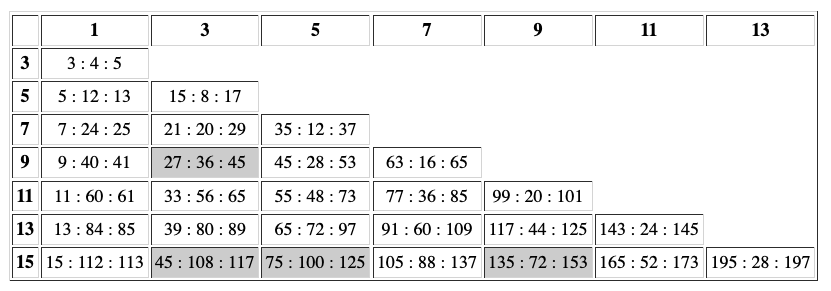
\includegraphics [scale=0.4] {triples_joyce.png} \end{center}

We can explain the first column from Joyce
\[ (3,4,5) \ \ \ (5,12,13) \ \ \ (7,24,25) \ \ \ (9,40,41) \]

using this graphic
\begin{center} 
\includegraphics [scale=0.4] {odd_numbers2.png} \end{center}

\[ n^2 + (2n + 1) = (n + 1)^2 \]
where $2n + 1$ is the count of dark blue squares in the top column plus the rightmost row.

Of course, this is just basic algebra.  Now, if that odd number is also a perfect square then we have that
\[ 2n + 1 = a^2 \]
so 
\[ (n + 1)^2 = n^2 + a^2 \]
Every odd number squared gives an odd perfect square:

\[ 3^2 = 9 \]
\[ 5^2 = 25 \]
\[ 7^2 = 49 \]

So every odd number ($\ge 3$) is the basis for one of the entries, and the other two values can be computed as
\[ b = \frac{a^2 - 1}{2}, \ \ \ \ c = b + 1 \]

We can also explain the first diagonal
\[ (8,15,17) \ \ \ (12,35,37) \ \ \ (16,63,65) \ \ \ (20,99,101) \]
The first value is $4n$ for $n = 2, 3, 4 \dots$.

The other two values are $4n^2 \pm 1$.  This works because
\[ (4n^2 + 1)^2 = (4n^2 - 1)^2 + (4n)^2 \]
The fourth powers cancel and the ones cancel and we have
\[ 8n^2 = -8n^2 + 16n^2 \]
which is correct.

Here is one set of primes I generated by brute-force search in Python with the constraints that either $a \le 50$ or $b \le 50$, no common factor, and none of the squares larger than $500$.

\begin{verbatim}
  3   4   5      5  12  13      7  24  25      8  15  17   
  9  40  41     11  60  61     12  35  37     13  84  85   
 15 112 113     16  63  65     17 144 145     19 180 181   
 20  21  29     20  99 101     21 220 221     23 264 265   
 24 143 145     25 312 313     27 364 365     28  45  53   
 28 195 197     29 420 421     31 480 481     32 255 257   
 33  56  65     36  77  85     36 323 325     39  80  89   
 40 399 401     44 117 125     44 483 485     48  55  73   
\end{verbatim}

\subsection*{opposite parity}
Euclid gave a formula for Pythagorean triples, which we will explain since he's so important in this book.

First of all, $a$ and $b$ are of opposite parity (one odd and one even) since if they were both even, then $c$ would be even so the triple would not be primitive.  They cannot both be odd either because then $c$ would be even and 
\[ (2x + 1)^2 + (2y + 1)^2 = (2z)^2 \]
\[ 4x^2 + 4x + 1 + 4y^2 + 4y + 1 = 4z^2 \]

The right-hand side is divisible by $4$ but the left is not.  This is impossible.  

Let $a$ be the odd value and $b$ the even one.
\[ a^2 + b^2 = c^2 \]
\[ a^2 = c^2 - b^2 = (c + b)(c - b) \]

\subsection*{perfect squares}

If we look at examples from above, say
\[ 15^2 = (17 + 8)(17 - 8) = 25 \cdot 9 \]
\[ 33^2 = (65 + 56)(65 - 56) = 121 \cdot 9 \]
\[ 55^2 = (73 + 48)(73 - 48) = 121 \cdot 25 \]
The two terms on the right are perfect squares.  This appears to always be true.

\subsection*{co-prime}

Next, $(c + b)$ and $(c - b)$ must be co-prime.

If $d$ were to divide both $(c + b)$ and $(c - b)$, then $d^2$ must divide $a^2$ and so $d$ divides $a$, but this doesn't help because we don't know about $b$ and $c$ individually ($3|9$ but not either $2$ or $7$).

Silverman argues that if $d$ were to divide both $(c + b)$ and $(c - b)$ then since
\[ (c + b) + (c - b) = 2c \]
\[ (c + b) - (c - b) = 2b \]

$d$ must divide both $2b$ and $2c$.  And since $b$ and $c$ are co-prime, $d$ must divide $2$ or $1$.  But $d$ also divides $a^2$ and $a^2$ is odd, so $d \ne 2$.  Hence $d = 1$.

\subsection*{conclusion}

The crucial observation is that if $(c + b)$ and $(c - b)$ are co-prime and their product is square, they must themselves be perfect squares.
\[ s^2 = c + b, \ \ \ \ \ \ t^2 = c - b \]
\[ \frac{s^2 + t^2}{2} = c, \ \ \ \ \ \ \frac{s^2 - t^2}{2} = b \]
\[ a^2 = s^2 t^2 \]
\[ a = st \]

\subsection*{Using the formula}

What we have derived above is often written slightly differently.  Let us rewrite this, but remembering that $b$ is even and $a$ is odd:

For every integer $m,n$, with $m > n$, a Pythagorean triple is given by
\[ a = m^2 - n^2 \ \ \ \ b = 2mn \ \ \ \ c = m^2 + n^2 \]

This works because
\[ (m^2 - n^2)^2 + (2mn)^2  =  (m^2 + n^2) \]
Canceling the fourth powers, we have
\[ -2m^2n^2 + 4m^2n^2 = 2m^2n^2 \]

So $c$ is a sum of squares.  For the first column $c$ is:
\[ 2^2 + 3^2, \ \ \ 3^2 + 4^2, \ \ \ 4^2 + 5^2 \]
 $a$ the difference, which is $1$.  For the second $c$ is
\[ 1^2 + 4^2, \ \ \ 1^2 + 6^2, \ \ \ 1^2 + 8^2, \ \ \ 1^2 + 10^2 \]

Clearly a number of patterns will be found.

This is discussed further in a separate chapter \hyperref[sec:pythagorean_triples]{\textbf{here}}.

\url{https://en.wikipedia.org/wiki/Pythagorean_triple#Enumeration_of_primitive_Pythagorean_triples}

A thousand years before Pythagoras, the Babylonians knew the triple $4601,4800,6649$.  It seems unlikely that they found this by random search.

\end{document}